\documentclass[xcolor=table]{beamer}
% generated by Madoko, version 1.1.6
%mdk-data-line={1}


\usepackage[heading-base={2},section-num={False},bib-label={hide},fontspec={True}]{madoko2}
%mdk-data-line={1;out\presentation.mdk:79}

    \ifbeamer\relax\else
      \providecommand{\usetheme}[2][]{}
      \providecommand{\usecolortheme}[2][]{}
      \providecommand{\usefonttheme}[2][]{}
      \providecommand{\pause}[1][]{}
      \providecommand{\AtBeginSection}[2][]{}
      \providecommand{\AtBeginSubsection}[2][]{}
      \providecommand{\AtBeginSubsubsection}[2][]{}
      \providecommand{\AtBeginPart}[2][]{}
      \providecommand{\AtBeginLecture}[2][]{}
      \providecommand{\theoremstyle}[2][]{}
      \makeatletter
      \def\newtheorem{\@ifstar\newtheoremx\newtheoremx}
      \makeatother
      \providecommand{\newtheoremx}[3][]{}{}
    \fi
%mdk-data-line={1;out\presentation.mdk:96}

    \ifbeamer\usetheme[]{singapore}\fi
\begin{document}



%mdk-data-line={9}
%mdk-data-line={9}
%mdk-data-line={10}
\mdxtitleblockstart{}
%mdk-data-line={10}
\mdxtitle{{\mdfontsize{3em}\mdline{10}VE370 Mid Review}}%mdk

%mdk-data-line={13}
\mdxtitlenote{\mdline{13}2018-10-28}%mdk
\mdxauthorstart{\Large{}
%mdk-data-line={18}
\mdxauthorname{{\mdfontsize{1.4em}\mdline{18}VE370 TA Group}}%mdk

%mdk-data-line={21}
\mdxauthoraddress{\mdline{21}UMJI-SJTU}%mdk
}\mdxauthorend\mdtitleauthorrunning{}{}\mdxtitleblockend%mdk

%mdk-data-line={12}
\begin{mdframe}%mdk

\frametitle{Content}\label{heading-sec-content}%mdk%mdk
\mdline{14}
\begin{mdtoc}%mdk

\begin{mdtocblock}%mdk

\mdtocitemx{sec-content}{\mdref{sec-content}{1.\hspace*{0.5em}Content}}%mdk

\mdtocitemx{sec-hw5-sample-solution}{\mdref{sec-hw5-sample-solution}{2.\hspace*{0.5em}HW5 Sample Solution}}%mdk

\begin{mdtocblock}%mdk

\mdtocitemx{sec-hw-5-1}{\mdref{sec-hw-5-1}{2.1.\hspace*{0.5em}HW 5. 1}}%mdk

\mdtocitemx{sec-hw-5-2-5-3}{\mdref{sec-hw-5-2-5-3}{2.2.\hspace*{0.5em}HW 5. 2 \& 5. 3}}%mdk

\mdtocitemx{sec-hw-5-4}{\mdref{sec-hw-5-4}{2.3.\hspace*{0.5em}HW 5. 4}}%mdk

\mdtocitemx{sec-hw-5-4}{\mdref{sec-hw-5-4}{2.4.\hspace*{0.5em}HW 5. 4}}%mdk

\mdtocitemx{sec-hw-5-5-5-6}{\mdref{sec-hw-5-5-5-6}{2.5.\hspace*{0.5em}HW 5. 5 \& 5. 6}}%mdk

\mdtocitemx{sec-hw-5-7}{\mdref{sec-hw-5-7}{2.6.\hspace*{0.5em}HW 5. 7}}%mdk

\mdtocitemx{sec-hw-5-8}{\mdref{sec-hw-5-8}{2.7.\hspace*{0.5em}HW 5. 8}}%mdk

\mdtocitemx{sec-hw-5-9}{\mdref{sec-hw-5-9}{2.8.\hspace*{0.5em}HW 5. 9}}%mdk

\mdtocitemx{sec-hw-5-10}{\mdref{sec-hw-5-10}{2.9.\hspace*{0.5em}HW 5. 10}}%mdk

\mdtocitemx{sec-hw-5-11}{\mdref{sec-hw-5-11}{2.10.\hspace*{0.5em}HW 5. 11}}%mdk

\mdtocitemx{sec-hw-5-12}{\mdref{sec-hw-5-12}{2.11.\hspace*{0.5em}HW 5. 12}}%mdk

\mdtocitemx{sec-hw-5-13}{\mdref{sec-hw-5-13}{2.12.\hspace*{0.5em}HW 5. 13}}%mdk
%mdk
\end{mdtocblock}%mdk

\mdtocitemx{sec-review}{\mdref{sec-review}{3.\hspace*{0.5em}Review}}%mdk

\begin{mdtocblock}%mdk

\mdtocitemx{sec-a-few-more-exercise}{\mdref{sec-a-few-more-exercise}{3.1.\hspace*{0.5em}A few more exercise}}%mdk
%mdk
\end{mdtocblock}%mdk
%mdk
\end{mdtocblock}%mdk
%mdk
\end{mdtoc}%mdk
%mdk
\end{mdframe}\label{sec-content}%mdk%mdk

%mdk-data-line={16}
\begin{mdframe}%mdk

\frametitle{HW5 Sample Solution}\label{heading-sec-hw5-sample-solution}%mdk%mdk
%mdk
\end{mdframe}\label{sec-hw5-sample-solution}%mdk%mdk

%mdk-data-line={20}
\begin{mdframe}%mdk

\frametitle{HW 5. 1}\label{heading-sec-hw-5-1}%mdk%mdk
\begin{mdpre}%mdk
\noindent~~{\mdcolor{navy}sw}~{\mdcolor{teal}R16},–{\mdcolor{purple}100}({\mdcolor{teal}R6})%mdk
\end{mdpre}\noindent\mdline{26}{\bfseries 4.16.1 (a)}\mdline{26} As  this  instruction  executes,  what  is  kept  in  each  register  located  between  two  pipeline  stages? 

%mdk-data-line={28}
\mdhr{}%mdk

%mdk-data-line={30}
\begin{itemize}%mdk
\begin{mdfragmented}%mdk

%mdk-data-line={30}
\item{}
%mdk-data-line={30}
\mdline{30}IF/ID: PC+4, instruction%mdk%mdk

%mdk-data-line={32}
\item{}
%mdk-data-line={32}
\mdline{32}ID/EX: PC+4, ReadData1(\mdline{32}\$\mdline{32}6), ReadData2(\mdline{32}\$\mdline{32}16), offset:\mdline{32} \mdline{32}-100(32b), Rs Rt field in this instruction, all control signals%mdk%mdk

%mdk-data-line={34}
\item{}
%mdk-data-line={34}
\mdline{34}EX/MEM: PC+4+offset, ReadData2(\mdline{34}\$\mdline{34}16), control signals for WB and MEM, Rs Rt field in this instruction, ALU result and ALU zero%mdk%mdk

%mdk-data-line={36}
\item{}
%mdk-data-line={36}
\mdline{36}MEM/WB: Control sinals for WB, ReadData from MEM, ALUresult, Selected Reg Destination%mdk%mdk
%mdk
\end{mdfragmented}%mdk
\end{itemize}%mdk
%mdk
\end{mdframe}\label{sec-hw-5-1}%mdk%mdk

%mdk-data-line={39}
\begin{mdframe}%mdk

\frametitle{HW 5. 2 \& 5. 3}\label{heading-sec-hw-5-2-5-3}%mdk%mdk

%mdk-data-line={41}
\noindent\mdline{41}{\bfseries 4.16.2 (a)}\mdline{41} Which  registers  need  to  be  read,  and  which  registers  are  actually read?%mdk

%mdk-data-line={44}
\mdhr{}%mdk

%mdk-data-line={46}
\begin{onlyenv}<+->%mdk
\begin{mdbmargintb}{}{\dimwidth{0.03}}%mdk
\noindent\mdline{46}need to be read: R16, R6; actually read: R16, R6%mdk
\end{mdbmargintb}%mdk
\end{onlyenv}%mdk

%mdk-data-line={49}
\mdline{49}{\bfseries 4.16.3 (a)}\mdline{49} What  does  this  instruction  do  in  the  EX  and  MEM  stages?%mdk

%mdk-data-line={52}
\mdhr{}%mdk

%mdk-data-line={53}
\begin{onlyenv}<+->%mdk

%mdk-data-line={54}
\noindent\mdline{54}EX:%mdk

%mdk-data-line={56}
\begin{itemize}[noitemsep,topsep=\mdcompacttopsep]%mdk

%mdk-data-line={56}
\item\mdline{56}Add the offset with the base address from R6%mdk

%mdk-data-line={57}
\item\mdline{57}Add PC+4 with the lower 16bits of instruction (useless)%mdk

%mdk-data-line={58}
\item\mdline{58}One reg destination is selected by mux (useless)%mdk
%mdk
\end{itemize}%mdk

%mdk-data-line={60}
\noindent\mdline{60}MEM:%mdk

%mdk-data-line={62}
\begin{itemize}[noitemsep,topsep=\mdcompacttopsep]%mdk

%mdk-data-line={62}
\item\mdline{62}Write the value of R16 into the target address in data memory%mdk
%mdk
\end{itemize}%mdk
%mdk
\end{onlyenv}%mdk
%mdk
\end{mdframe}\label{sec-hw-5-2-5-3}%mdk%mdk

%mdk-data-line={70}
\begin{mdframe}%mdk

\frametitle{HW 5. 4}\label{heading-sec-hw-5-4}%mdk%mdk
\begin{mdpre}%mdk
\noindent{\mdcolor{teal}LOOP}:\\
~~{\mdcolor{navy}add}~\$1,~\$2,~\$1\\
~~{\mdcolor{navy}lw}~~\$2,~{\mdcolor{purple}0}(\$1)\\
~~{\mdcolor{navy}lw}~~\$2,~{\mdcolor{purple}16}(\$2)\\
~~{\mdcolor{navy}slt}~\$1,~\$2,~\$5\\
~~{\mdcolor{navy}beq}~\$1,~\$9,~{\mdcolor{teal}LOOP}%mdk
\end{mdpre}\noindent\mdline{80}{\bfseries 4.16.4(b)}\mdline{80} Show  a  pipeline  execution  diagram  for  the  third  iteration  of  this  loop,  from  the  cycle  in  which  we  fetch  the  first  instruction  of  that  iteration  up  to  (but  not  including)  the  cycle  in  which  we  can  fetch  the  first  instruction  of  the  next  iteration.  Show  all  instructions  that  are  in  the  pipeline  during  these  cycles  (not  just  those  from  the  third  iteration).
%mdk
\end{mdframe}\label{sec-hw-5-4}%mdk%mdk

%mdk-data-line={82}
\begin{mdframe}%mdk

\frametitle{HW 5. 4}\label{heading-sec-hw-5-4}%mdk%mdk

%mdk-data-line={84}
\noindent\mdline{84}Solution:%mdk
\begin{mdtabular}{2}{\dimeval{(\linewidth)/2}}{0pt}%mdk
\begin{tabular}{ll}

%mdk-data-line={87}
\begin{mdcolumn}%mdk
\begin{mdblock}{width=\dimavailable}%mdk
\begin{mdpre}%mdk
\noindent~~~~~~~~~~~~~~{\mdcolor{navy}add}~\$1,~\$1,~\$2\\
~~~~~~~~~~~~~~{\mdcolor{navy}lw}~~\$1,~{\mdcolor{purple}0}(\$1)\\
~~~~~~~~~~~~~~{\mdcolor{navy}lw}~~\$1,~{\mdcolor{purple}0}(\$1)\\
~~~~~~~~~~~~~~{\mdcolor{navy}beq}~\$1,~\$0,~{\mdcolor{teal}LOOP}\\
{\mdcolor{teal}LOOP}:~({\mdcolor{purple}3}rd)~~~{\mdcolor{navy}lw}~~\$1,~{\mdcolor{purple}0}(\$1)\\
~~~~~~~~~~~~~~{\mdcolor{navy}add}~\$1,~\$1,~\$2\\
~~~~~~~~~~~~~~{\mdcolor{navy}lw}~~\$1,~{\mdcolor{purple}0}(\$1)\\
~~~~~~~~~~~~~~{\mdcolor{navy}lw}~~\$1,~{\mdcolor{purple}0}(\$1)\\
~~~~~~~~~~~~~~{\mdcolor{navy}beq}~\$1,~\$0,~{\mdcolor{teal}LOOP}\\
{\mdcolor{teal}LOOP}:~({\mdcolor{purple}4}th)~~~{\mdcolor{navy}lw}~~\$1,~{\mdcolor{purple}0}(\$1)%mdk
\end{mdpre}%mdk
\end{mdblock}%mdk
\end{mdcolumn}%mdk
&
%mdk-data-line={101}
\begin{mdcolumn}%mdk
\begin{mdblock}{width=\dimavailable}%mdk
\begin{mdpre}%mdk
\noindent{\mdcolor{teal}WB}\\
{\mdcolor{teal}MEM}~{\mdcolor{teal}WB}\\
{\mdcolor{teal}EX}~~{\mdcolor{teal}MEM}~{\mdcolor{teal}WB}\\
{\mdcolor{teal}ID}~~{\mdcolor{teal}EX}~~{\mdcolor{teal}MEM}~{\mdcolor{teal}WB}\\
{\mdcolor{teal}IF}~~{\mdcolor{teal}ID}~~{\mdcolor{teal}EX}~~{\mdcolor{teal}MEM}~{\mdcolor{teal}WB}\\
~~~~{\mdcolor{teal}EX}~~{\mdcolor{teal}ID}~~{\mdcolor{teal}EX}~~{\mdcolor{teal}MEM}~{\mdcolor{teal}WB}\\
~~~~~~~~{\mdcolor{teal}IF}~~{\mdcolor{teal}ID}~~{\mdcolor{teal}EX}~~{\mdcolor{teal}MEM}\\
~~~~~~~~~~~~{\mdcolor{teal}IF}~~{\mdcolor{teal}ID}~~{\mdcolor{teal}EX}\\
~~~~~~~~~~~~~~~~{\mdcolor{teal}IF}~~{\mdcolor{teal}ID}\\
~~~~~~~~~~~~~~~~~~~~{\mdcolor{teal}IF}%mdk
\end{mdpre}%mdk
\end{mdblock}%mdk
\end{mdcolumn}%mdk
\\
\end{tabular}\end{mdtabular}
%mdk
\end{mdframe}\label{sec-hw-5-4}%mdk%mdk

%mdk-data-line={117}
\begin{mdframe}%mdk

\frametitle{HW 5. 5 \& 5. 6}\label{heading-sec-hw-5-5-5-6}%mdk%mdk

%mdk-data-line={119}
\noindent\mdline{119}{\bfseries 4.16.5(b)}\mdline{119} How  often  (as  a  percentage  of  all  cycles)  do  we  have  a  cycle  in  which  all  five  pipeline  stages  are  doing  useful  work?%mdk

%mdk-data-line={121}
\mdhr{}%mdk

%mdk-data-line={123}
\begin{onlyenv}<+->%mdk
\noindent\mdline{123}\mdcode{{\mdcolor{navy}lw}}\mdline{123} fully takes use of all stages; \mdline{123}\mdcode{{\mdcolor{navy}add}}\mdline{123} does no useful work in MEM; \mdline{123}\mdcode{{\mdcolor{navy}beq}}\mdline{123} does no useful work in WB%mdk
\end{onlyenv}%mdk

%mdk-data-line={126}
\begin{onlyenv}<+->%mdk
\begin{mdbmargintb}{}{\dimwidth{0.03}}%mdk
\mdline{126}Only the first three clocks out of five are fully used.%mdk
\end{mdbmargintb}%mdk
\end{onlyenv}%mdk

%mdk-data-line={129}
\mdline{129}{\bfseries 4.16.6(b)}\mdline{129} At  the  start  of  the  cycle  in  which  we  fetch  the  first  instruction  of  the  third  iteration  of  this  loop,  what  is  stored  in  the  IF/ID  register?%mdk

%mdk-data-line={131}
\mdhr{}%mdk

%mdk-data-line={133}
\begin{itemize}[noitemsep,topsep=\mdcompacttopsep]%mdk
\begin{mdfragmented}%mdk

%mdk-data-line={133}
\item\mdline{133}Fetched instruction from 2nd iteration \mdline{133}\mdcode{{\mdcolor{navy}beq}~\$1,~\$0,~{\mdcolor{teal}LOOP}}\mdline{133}%mdk

%mdk-data-line={134}
\item\mdline{134}PC+4%mdk
%mdk
\end{mdfragmented}%mdk
\end{itemize}%mdk
%mdk
\end{mdframe}\label{sec-hw-5-5-5-6}%mdk%mdk

%mdk-data-line={139}
\begin{mdframe}%mdk

\frametitle{HW 5. 7}\label{heading-sec-hw-5-7}%mdk%mdk

%mdk-data-line={140}
\noindent\mdline{140}4.17.3 Problems  in  this  exercise  assume  that  instructions  executed  by  a  pipelined  processor  are  broken  down  as  follows:%mdk

%mdk-data-line={142}
\begin{mdcenter}%mdk

%mdk-data-line={143}
\noindent\mdline{143}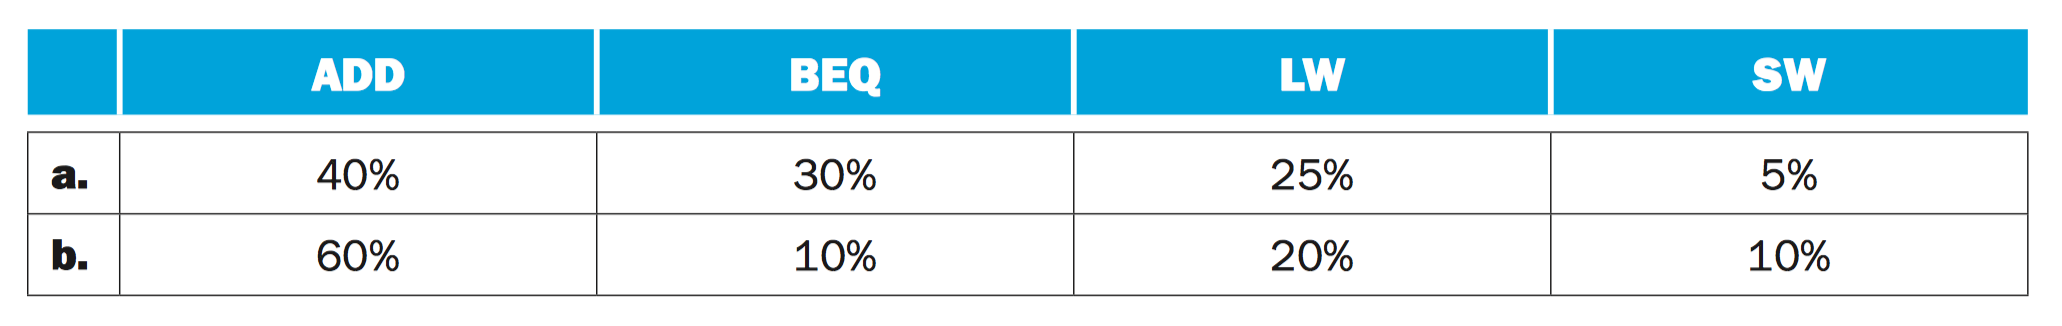
\includegraphics[keepaspectratio=true,width=\dimmin{}{\dimwidth{1.00}}]{images/Screen-Shot-2018-10-27-at-9.15.17-PM}{}\mdline{143}%mdk
%mdk
\end{mdcenter}%mdk

%mdk-data-line={149}
\noindent\mdline{149}Assuming  there  are  no  stalls,  how  often  (percentage  of  all  cycles) do we use the data memory?%mdk

%mdk-data-line={151}
\mdhr{}%mdk

%mdk-data-line={153}
\begin{onlyenv}<+->%mdk

%mdk-data-line={154}
\noindent\mdline{154}The percentage we use DMEM is just the sum of percentages of \mdline{154}\mdcode{{\mdcolor{navy}sw}}\mdline{154} and \mdline{154}\mdcode{{\mdcolor{navy}lw}}\mdline{154}.%mdk

%mdk-data-line={156}
\begin{enumerate}[noitemsep,topsep=\mdcompacttopsep,label=\alph*.]%mdk

%mdk-data-line={156}
\item\mdline{156}25\%+5\%  = 30\%%mdk

%mdk-data-line={157}
\item\mdline{157}20\%+10\% = 30\%%mdk
%mdk
\end{enumerate}%mdk
%mdk
\end{onlyenv}%mdk
%mdk
\end{mdframe}\label{sec-hw-5-7}%mdk%mdk

%mdk-data-line={162}
\begin{mdframe}%mdk

\frametitle{HW 5. 8}\label{heading-sec-hw-5-8}%mdk%mdk

%mdk-data-line={164}
\begin{mdcenter}%mdk

%mdk-data-line={165}
\noindent\mdline{165}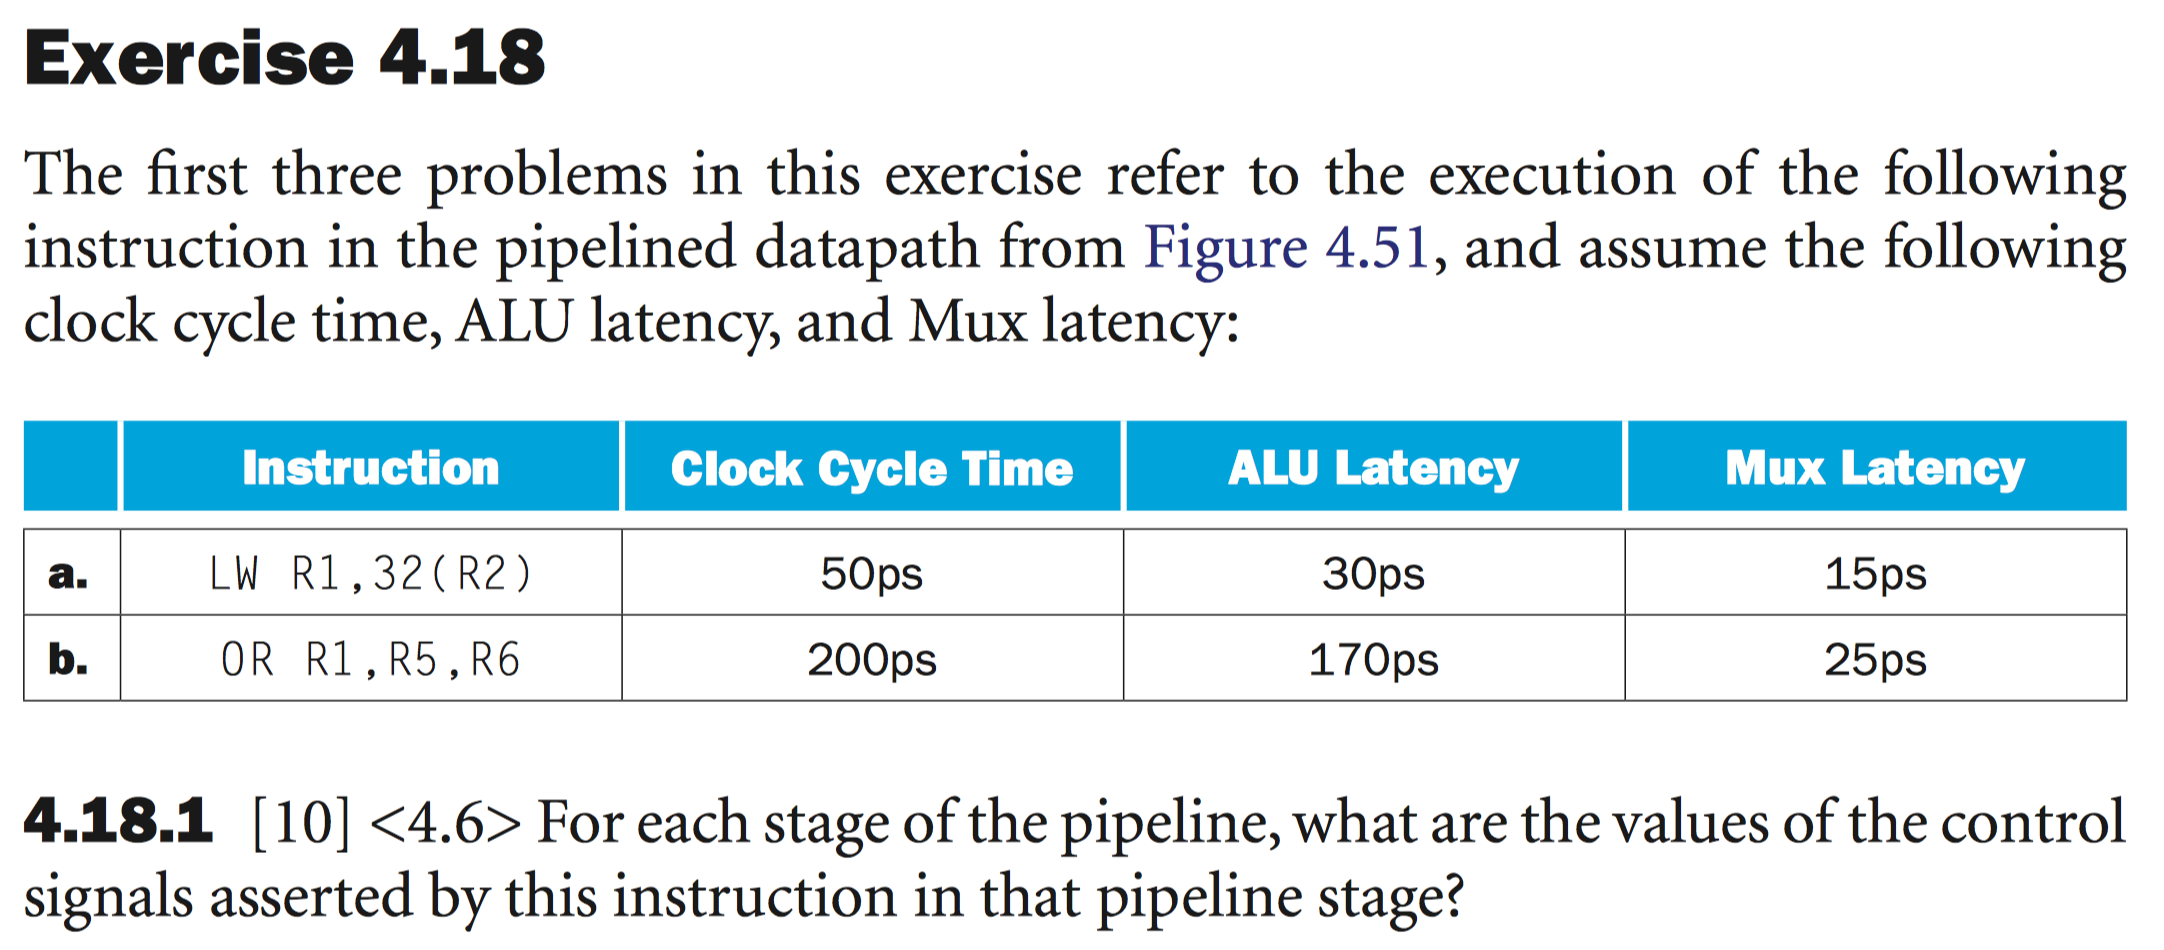
\includegraphics[keepaspectratio=true,width=\dimmin{}{\dimwidth{1.00}}]{images/Screen-Shot-2018-10-27-at-9.20.45-PM}{}\mdline{165}%mdk
%mdk
\end{mdcenter}%mdk

%mdk-data-line={170}
\noindent\mdline{170}{\bfseries 4.18.1 (b)}\mdline{170}%mdk

%mdk-data-line={172}
\begin{itemize}[noitemsep,topsep=\mdcompacttopsep]%mdk
\begin{mdfragmented}%mdk

%mdk-data-line={172}
\item\mdline{172}Ex: ALUop: 00; RegDst: 0; ALUSrc: 1%mdk

%mdk-data-line={173}
\item\mdline{173}MEM: Branch: 0; MEMWrite: 0; MEMRead: 1%mdk

%mdk-data-line={174}
\item\mdline{174}MemtoReg: 0; RegWrite: 1%mdk
%mdk
\end{mdfragmented}%mdk
\end{itemize}%mdk
%mdk
\end{mdframe}\label{sec-hw-5-8}%mdk%mdk

%mdk-data-line={177}
\begin{mdframe}%mdk

\frametitle{HW 5. 9}\label{heading-sec-hw-5-9}%mdk%mdk

%mdk-data-line={179}
\noindent\mdline{179}{\bfseries 4.18.3 (b)}\mdline{179} What  is  the  value  of  the  PCSrc  signal  for  this  instruction?  This  signal  is generated  early  in  the  MEM  stage  (only  a  single  AND  gate).  What  would  be  a  reason  in  favor  of  doing  this  in  the  EX  stage?  What  is  the  reason  against  doing  it  in  the  EX  stage?%mdk

%mdk-data-line={181}
\mdhr{}%mdk

%mdk-data-line={183}
\noindent\mdline{183}PCsrc = 0.%mdk

%mdk-data-line={185}
\begin{itemize}[noitemsep,topsep=\mdcompacttopsep]%mdk

%mdk-data-line={185}
\item\mdline{185}Reason for in EX: one clock cycle earlier to select the correct result of pc (useful for branch instructions)%mdk

%mdk-data-line={186}
\item\mdline{186}Reason for in MEM: PCsrc is dependent on ALUzero and need further AND calculation. May exceed the cycle length.%mdk
%mdk
\end{itemize}%mdk
%mdk
\end{mdframe}\label{sec-hw-5-9}%mdk%mdk

%mdk-data-line={191}
\begin{mdframe}%mdk

\frametitle{HW 5. 10}\label{heading-sec-hw-5-10}%mdk%mdk

%mdk-data-line={193}
\noindent\mdline{193}Problems in this exercise refer to the following instruction sequences (b)%mdk

%mdk-data-line={195}
\begin{mdblock}{width=\dimwidth{0.50}}%mdk
\begin{mdpre}%mdk
\noindent{\mdcolor{teal}I1}:~~{\mdcolor{navy}add}~\$1,~\$2,~\$1\\
{\mdcolor{teal}I2}:~~{\mdcolor{navy}lw}~~\$2,~{\mdcolor{purple}0}(\$1)\\
{\mdcolor{teal}I3}:~~{\mdcolor{navy}lw}~~\$1,~{\mdcolor{purple}4}(\$1)\\
{\mdcolor{teal}I4}:~~{\mdcolor{navy}or}~~\$3,~\$1,~\$2%mdk
\end{mdpre}%mdk
\end{mdblock}%mdk

%mdk-data-line={204}
\noindent\mdline{204}{\bfseries 4.20.1(a)}\mdline{204}  Find  all  data  dependences  in  this  instruction  sequence.%mdk

%mdk-data-line={206}
\mdhr{}%mdk

%mdk-data-line={208}
\begin{itemize}%mdk
\begin{mdfragmented}%mdk

%mdk-data-line={208}
\item{}
%mdk-data-line={208}
\mdline{208}ReadAfterWrite: I1\mdline{208} \mdline{208}- I2 I3 I4(\mdline{208}\$\mdline{208}1), I2\mdline{208} \mdline{208}- I4(\mdline{208}\$\mdline{208}2), I3\mdline{208} \mdline{208}- I4(\mdline{208}\$\mdline{208}1)%mdk%mdk

%mdk-data-line={210}
\item{}
%mdk-data-line={210}
\mdline{210}WriteAfterRead: I1\mdline{210} \mdline{210}- I2(\mdline{210}\$\mdline{210}2), I1\mdline{210} \mdline{210}- I3(\mdline{210}\$\mdline{210}1)%mdk%mdk

%mdk-data-line={212}
\item{}
%mdk-data-line={212}
\mdline{212}WriteAfterWrite: I1\mdline{212} \mdline{212}- I3(\mdline{212}\$\mdline{212}1)%mdk%mdk
%mdk
\end{mdfragmented}%mdk
\end{itemize}%mdk
%mdk
\end{mdframe}\label{sec-hw-5-10}%mdk%mdk

%mdk-data-line={215}
\begin{mdframe}%mdk

\frametitle{HW 5. 11}\label{heading-sec-hw-5-11}%mdk%mdk

%mdk-data-line={217}
\begin{mdblock}{width=\dimwidth{0.50}}%mdk
\begin{mdpre}%mdk
\noindent~~{\mdcolor{navy}add}~\$1,~\$2,~\$1\\
~~{\mdcolor{navy}lw}~~\$2,~{\mdcolor{purple}0}(\$1)\\
~~{\mdcolor{navy}lw}~~\$1,~{\mdcolor{purple}4}(\$1)\\
~~{\mdcolor{navy}or}~~\$3,~\$1,~\$2%mdk
\end{mdpre}%mdk
\end{mdblock}%mdk

%mdk-data-line={226}
\noindent\mdline{226}{\bfseries 4.20.3(a)}\mdline{226} To  reduce  clock  cycle  time,  we  are  considering  a  split  of the MEM  stage  into  two  stages. Find  all  hazards  in  this  instruction  sequence  for  this  6-stage  pipeline with and then without forwarding.%mdk

%mdk-data-line={228}
\mdhr{}%mdk

%mdk-data-line={230}
\noindent\mdline{230}The only difference is that originally load-use harzard only affects the very next instruction with RAW dependency while in this 6-stage version, it will affect next 2 intructions.%mdk

%mdk-data-line={232}
\begin{itemize}[noitemsep,topsep=\mdcompacttopsep]%mdk

%mdk-data-line={232}
\item\mdline{232}With Forwarding: I2\mdline{232} \mdline{232}- I4(\mdline{232}\$\mdline{232}2) (not exists in 5-stage), I3\mdline{232} \mdline{232}- I4(\mdline{232}\$\mdline{232}2)%mdk

%mdk-data-line={233}
\item\mdline{233}Without Forwarding: I1\mdline{233} \mdline{233}- I2 I3(\mdline{233}\$\mdline{233}1), I2\mdline{233} \mdline{233}- I4(\mdline{233}\$\mdline{233}2), I3\mdline{233} \mdline{233}- I4(\mdline{233}\$\mdline{233}1)%mdk
%mdk
\end{itemize}%mdk
%mdk
\end{mdframe}\label{sec-hw-5-11}%mdk%mdk

%mdk-data-line={236}
\begin{mdframe}%mdk

\frametitle{HW 5. 12}\label{heading-sec-hw-5-12}%mdk%mdk

%mdk-data-line={238}
\noindent\mdline{238} We assume that all  values  in  data  memory  are  zeroes  and  that  registers have  the  following  initial  values:%mdk
\begin{mdtabular}{2}{\dimeval{(\linewidth-\dimwidth{0.75})/1}}{0pt}%mdk
\begin{tabular}{ll}

%mdk-data-line={241}
\begin{mdcolumn}%mdk
\begin{mdblock}{vertical-align=bottom,width=\dimwidth{0.75}}%mdk
%mdk-data-line={242}
\noindent\mdline{242}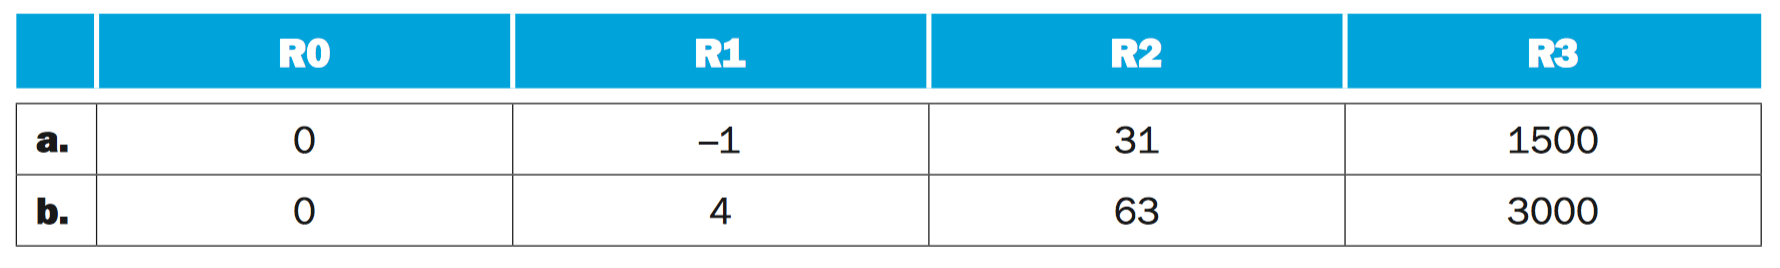
\includegraphics[keepaspectratio=true,width=\dimmin{}{\dimwidth{1.00}}]{images/5_12}{}\mdline{242}%mdk%mdk
\end{mdblock}%mdk
\end{mdcolumn}%mdk
&
%mdk-data-line={245}
\begin{mdcolumn}%mdk
\begin{mdblock}{vertical-align=top,width=\dimavailable}%mdk
\begin{mdpre}%mdk
\noindent~~{\mdcolor{navy}add}~\$1,~\$2,~\$1\\
~~{\mdcolor{navy}lw}~~\$2,~{\mdcolor{purple}0}(\$1)\\
~~{\mdcolor{navy}lw}~~\$1,~{\mdcolor{purple}4}(\$1)\\
~~{\mdcolor{navy}or}~~\$3,~\$1,~\$2%mdk
\end{mdpre}%mdk
\end{mdblock}%mdk
\end{mdcolumn}%mdk
\\
\end{tabular}\end{mdtabular}

%mdk-data-line={255}
\noindent\mdline{255}{\bfseries 4.20.5(a)}\mdline{255}  If  we  assume  forwarding  will  be  implemented  when  we  design  the  hazard  detection  unit,  but  then  we  forget  to  actually  implement  forwarding what  are  the  final  register  values  after  this  instruction  sequence?%mdk

%mdk-data-line={257}
\mdhr{}%mdk

%mdk-data-line={259}
\noindent\mdline{259}Without forwarding, the written reg can only be updated after two cycles of the execution.%mdk

%mdk-data-line={261}
\begin{mdcenter}%mdk
\mdline{261}\$\mdline{261}1 = 0; \mdline{261}\$\mdline{261}2 = 0; \mdline{261}\$\mdline{261}3 = 30\mdline{261}$\lor$\mdline{261}31 = 31\mdline{261}\mdsub{dec}%mdk
\end{mdcenter}%mdk
%mdk
\end{mdframe}\label{sec-hw-5-12}%mdk%mdk

%mdk-data-line={264}
\begin{mdframe}%mdk

\frametitle{HW 5. 13}\label{heading-sec-hw-5-13}%mdk%mdk
\begin{mdtabular}{2}{\dimeval{(\linewidth-\dimwidth{0.75})/1}}{0pt}%mdk
\begin{tabular}{ll}

%mdk-data-line={267}
\begin{mdcolumn}%mdk
\begin{mdblock}{vertical-align=bottom,width=\dimwidth{0.75}}%mdk
%mdk-data-line={268}
\noindent\mdline{268}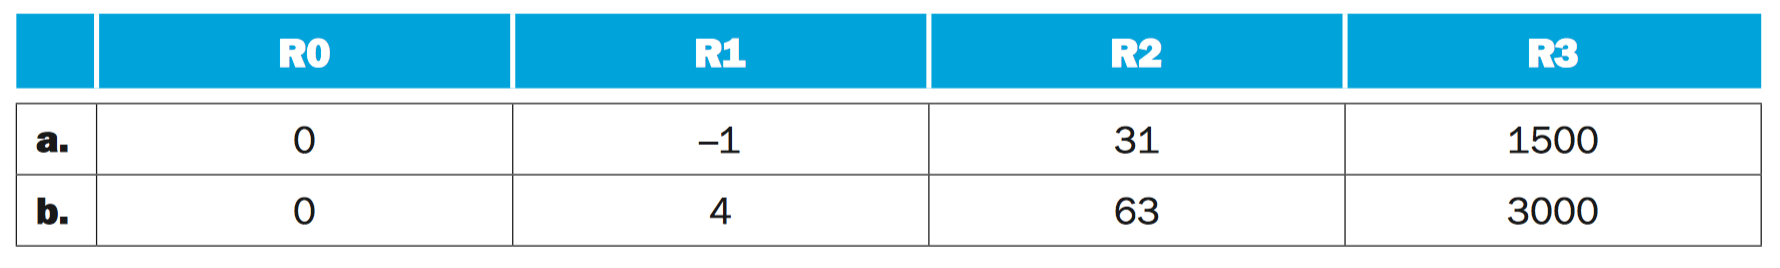
\includegraphics[keepaspectratio=true,width=\dimmin{}{\dimwidth{1.00}}]{images/5_12}{}\mdline{268}%mdk%mdk
\end{mdblock}%mdk
\end{mdcolumn}%mdk
&
%mdk-data-line={271}
\begin{mdcolumn}%mdk
\begin{mdblock}{vertical-align=top,width=\dimavailable}%mdk
\begin{mdpre}%mdk
\noindent~~{\mdcolor{navy}add}~\$1,~\$2,~\$1\\
~~{\mdcolor{navy}lw}~~\$2,~{\mdcolor{purple}0}(\$1)\\
~~{\mdcolor{navy}lw}~~\$1,~{\mdcolor{purple}4}(\$1)\\
~~{\mdcolor{navy}or}~~\$3,~\$1,~\$2%mdk
\end{mdpre}%mdk
\end{mdblock}%mdk
\end{mdcolumn}%mdk
\\
\end{tabular}\end{mdtabular}

%mdk-data-line={281}
\noindent\mdline{281}{\bfseries 4.20.6(a)}\mdline{281} Add  NOPs  sequence  to  ensure  correct  execution  in  spite  of  missing  support  for  forwarding.%mdk

%mdk-data-line={283}
\mdhr{}%mdk

%mdk-data-line={284}
\begin{mdcenter}%mdk
\begin{mdpre}%mdk
\begin{mdblock}{width=\dimwidth{0.50}}%mdk
\noindent~~{\mdcolor{navy}add}~\$1,~\$2,~\$1\\
~~{\mdcolor{teal}NOP}\\
~~{\mdcolor{teal}NOP}\\
~~{\mdcolor{navy}lw}~~\$2,~{\mdcolor{purple}0}(\$1)\\
~~{\mdcolor{navy}lw}~~\$1,~{\mdcolor{purple}4}(\$1)\\
~~{\mdcolor{teal}NOP}\\
~~{\mdcolor{teal}NOP}\\
~~{\mdcolor{navy}or}~~\$3,~\$1,~\$2%mdk
\end{mdblock}%mdk
\end{mdpre}%mdk
\end{mdcenter}%mdk
%mdk
\end{mdframe}\label{sec-hw-5-13}%mdk%mdk

%mdk-data-line={299}
\begin{mdframe}%mdk

\frametitle{Review}\label{heading-sec-review}%mdk%mdk
%mdk
\end{mdframe}\label{sec-review}%mdk%mdk

%mdk-data-line={301}
\begin{mdframe}%mdk

\frametitle{A few more exercise}\label{heading-sec-a-few-more-exercise}%mdk%mdk
%mdk
\end{mdframe}\label{sec-a-few-more-exercise}%mdk%mdk%mdk%mdk%mdk


\end{document}
